\documentclass[unicode,12pt,aspectratio=169, dvipdfmx]{beamer}
\usepackage{bxdpx-beamer}
\usetheme[progressbar=frametitle]{metropolis}
\renewcommand{\kanjifamilydefault}{\gtdefault}%既定をゴシック体に
\usepackage{bm}
% \usepackage{color}
%\usepackage{graphicx}


% タイトル、著者、日付の情報
\title{Optimizing IoT Data Collection for Federated Learning Under Constraint of Wireless Bandwidth}
\author{竹本志恩}
\date{\today}
% \subtitle{latexで作成}
\date[]{\today}
\institute{INIAD}
\subject{latexでレジュメを作る}
% \keywords{LaTeX2e,Beamer,Presentation}
\AtBeginSection[]{
    \frame{{目次}\tableofcontents[currentsection, hideallsubsections]} %目次スライド
}




\begin{document}
% タイトルスライド
    \frame{\maketitle}
    \section{1. はじめに}
    \begin{frame}{書誌情報}
        \begin{columns}
            \begin{column}{.8\linewidth}
                \begin{itemize}
                    \item 題名
                    \begin{itemize}
                        \item Optimizing IoT Data Collection for Federated Learning Under Constraint of Wireless Bandwidth
                    \end{itemize}
                    
                    \item 発表日
                    \begin{itemize}
                        \item 20 August 2024
                    \end{itemize}

                    \item 著者
                    \begin{itemize}
                        \item Tajiri Kengo, Ryoichi Kawahara
                    \end{itemize}

                    % \item 会議名
                    \item 論文誌名
                    \begin{itemize}
                        \item IEEE
                    \end{itemize}
                    % \item 会議: IEEE ICC 2024
                \end{itemize}          
            \end{column}
        \end{columns}
    \end{frame}

    \begin{frame}{どんな研究?}
        \begin{columns}
            \begin{column}{.8\linewidth}
                \begin{itemize}
                    \item IoTでのデータ利活用のため
                    \item 帯域幅制約の下で実験を行い
                    \item 提案手法によるFL$^{*}$の精度向上を確認
                    
                    \small {* Federated Learning, 連合学習}
                \end{itemize}          
            \end{column}
        \end{columns}
    \end{frame}

    % \section{2. 前提の共有}

    % \begin{frame}{数理最適化}
    %     \begin{columns}
    %         \begin{column}[T]{.7\linewidth}
    %             \begin{itemize}
    %                 \item 現象などをモデル化
    %                 \item 何らかの項目を最小あるいは最大にする
    %                 \item 
    %                 \begin{itemize}
    %                     \item 統合とパラメータサーバが存在
    %                     \item 各パラメータサーバは個別にデータを保持
    %                 \end{itemize}    
    %             \end{itemize}          
    %         \end{column}
    %         \begin{column}[T]{.5\linewidth}
    %             \begin{itemize}
    %                 \item 図を入れる
    %             \end{itemize}
    %         \end{column}
    %     \end{columns}
    % \end{frame}

    \section{2. 動機}
    \begin{frame}{背景}
        \begin{columns}
            \begin{column}[T]{.6\linewidth}
                \begin{itemize}
                    \item IoTの普及に伴いデバイスが増加
                    \item 従来のデータ集約・分析が困難に
                    \begin{itemize}
                        \item 総データ生成量の増加
                        \item 利用帯域・計算コストの増加
                    \end{itemize}
                    \item Federated Learningに着目
                    \begin{itemize}
                        \item 分散機械学習の一手法
                        \item データを分散し,上記の問題を解決
                    \end{itemize}
                \end{itemize}
            \end{column}
            % \begin{column}[T]{.5\linewidth}
            % \end{column}
        \end{columns}
    \end{frame}


    \begin{frame}{Federated Learningとは}
        \begin{columns}
            \begin{column}[T]{.7\linewidth}
                \begin{itemize}
                    \item 連合学習, FL
                    \begin{itemize}
                        \item 分散的に学習する手法の一つ
                        \item 各サーバはデータを持ち,学習
                        \item 学習結果をあるサーバで集約
                        \item 統合,パラメータサーバが存在
                    \end{itemize}  
                    \item 大まかな流れ
                    \begin{itemize}
                        \item 統合サーバからモデルを配布
                        \item 各パラメータサーバはローカルデータで学習
                        \item モデルのパラメータを統合サーバで集約
                        \item モデルを更新し再配布
                        \item 一連の流れを繰り返す
                    \end{itemize}    
                \end{itemize}          
            \end{column}
            \begin{column}[T]{.5\linewidth}
                    \begin{center}
                        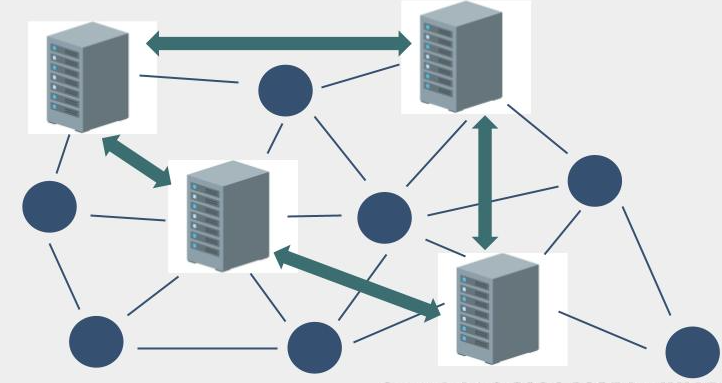
\includegraphics[scale=0.3]{figures/fl.png}
                        \scriptsize{FLのイメージ}
                    \end{center}
            \end{column}
        \end{columns}
    \end{frame}


    \begin{frame}{課題}
        \begin{columns}
            \begin{column}[T]{.7\linewidth}
                \begin{itemize}
                    \item IoTデバイス(ID)から基地局(BS)へのデータ転送
                    \item 想定されるシナリオ
                    \begin{itemize}
                        \item 各BSはサーバとIDを所持
                        \item BSにIDからデータを送信
                        \item サーバの持つデータでモデルを学習
                    \end{itemize}
                    \item FLの精度
                    \begin{itemize}
                        \item サーバの持つデータの量と分布が影響
                        \item 量と分布は制約の下決めた伝送先に依存
                        \item IDからどのBSに送信するかが重要
                    \end{itemize}
                    \item 帯域幅制約下でFLの精度を向上
                        \begin{itemize}
                            \item 制約により送信先が限定
                            \item その中で最適なBSを決定
                        \end{itemize}
                \end{itemize}
            \end{column}
            \begin{column}[T]{.5\linewidth}
                \begin{center}
                    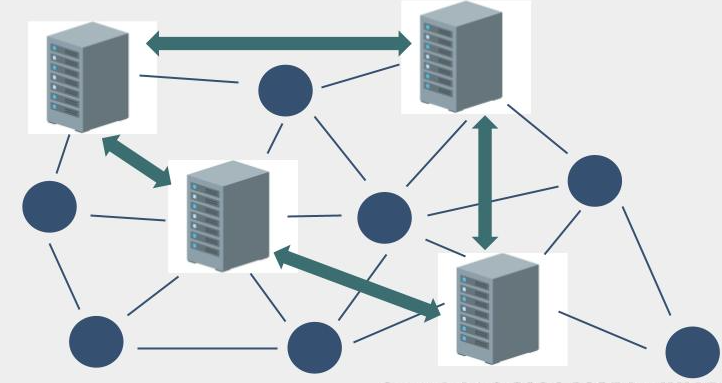
\includegraphics[scale=0.3]{figures/fl.png}
                    \scriptsize{再掲}
                \end{center}
        \end{column}
        \end{columns}
    \end{frame}



    \section{3. 手法}
    \begin{frame}{手法の概要}
        \begin{columns}
            \begin{column}[]{.8\linewidth}
                \begin{itemize}
                    \item やること
                    \begin{itemize}
                        \item 帯域制約の下
                        \item FLの精度を最大化するような
                        \item 最適化問題を解く
                    \end{itemize}
                    \item 解法
                    \begin{itemize}
                        \item 遺伝的アルゴリズム
                        \item IDからどのBSにデータを送信するか決定
                        % \begin{itemize}
                        %     \item データの送信に着目
                        %     \item パラメータの方は気にしない?
                        % \end{itemize}
                    \end{itemize}
                    \item 実験
                    \begin{itemize}
                        \item 提案手法とナイーブを比較
                        \item 数値実験
                        \item 仮想クラスタでの学習
                        \begin{itemize}
                            \item 三種類の機械学習モデルで比較
                        \end{itemize}
                    \end{itemize}
                \end{itemize}
            \end{column}
        \end{columns}
    \end{frame}

    \begin{frame}{OFDMA}
        \begin{columns}
            \begin{column}[T]{.7\linewidth}
                \begin{itemize}
                    \item 周波数を分割し割当て
                    \item 単一の通信路で複数のやり取りが可能に
                    \item リソースブロック(RB)という単位で管理?
                    \begin{itemize}
                        \item データのやり取りに用いるそういう塊がある
                    \end{itemize}    
                \end{itemize}          
            \end{column}
            % \begin{column}[T]{.5\linewidth}
            %     \begin{itemize}
            %         \item 図を入れる
            %     \end{itemize}
            % \end{column}
        \end{columns}
    \end{frame}

    \begin{frame}{問題設定}
        \begin{columns}
            \begin{column}[T]{.7\linewidth}
                \begin{itemize}
                    \item ID: $I = {\{1, 2, ..., N\}}$
                    \item BS: $B = {\{1, 2, ..., M\}}$
                    \item 単位時間あたりのデータ生成量: $\lambda_{i}$
                    \item 一回の学習におけるデータ収集量: $T$
                    \item RB: $R = {\{1, 2, ..., K\}}$
                \end{itemize}          
            \end{column}
            % \begin{column}[T]{.5\linewidth}
            %     \begin{itemize}
            %         \item 図を入れる
            %     \end{itemize}
            % \end{column}
        \end{columns}
    \end{frame}


    \begin{frame}{制約条件1-4}
        \begin{columns}
            \begin{column}[T]{.6\linewidth}
                \begin{itemize}
                    \item IDがRBを使ってBSにデータを渡すよ,というのを定義
                    \item IDに対してBSは0個でもいい
                    \begin{itemize}
                        \item 送らないIDの存在を許容
                    \end{itemize}    
                    \item 伝送時にはBSとRBが同じだけ必要
                    \item RBはIDに一つのみ割り当て
                    \begin{itemize}
                        \item 送らない場合があるので不等式
                    \end{itemize}    
                \end{itemize}          
            \end{column}
            \begin{column}[T]{.5\linewidth}
                \begin{center}
                    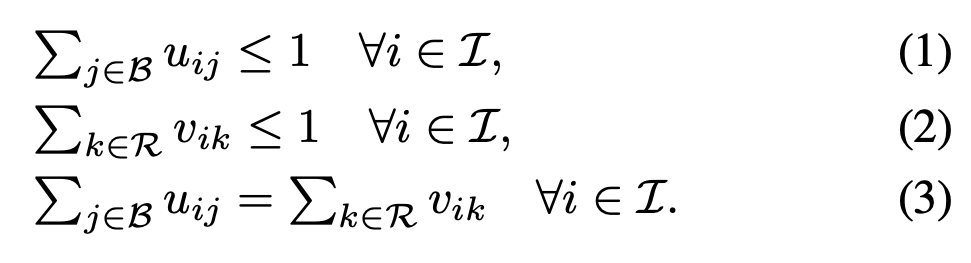
\includegraphics[scale=0.4]{figures/eq1-3.png}
                    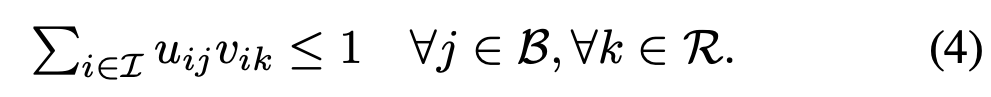
\includegraphics[scale=0.4]{figures/eq4.png}
                \end{center}
        \end{column}
        \end{columns}
    \end{frame}


    \begin{frame}{制約条件5-8}
        \begin{columns}
            \begin{column}[T]{.5\linewidth}
                \begin{itemize}
                    \item 無線接続の帯域幅を定義
                    \item 7が単純にID~BS間の帯域幅
                    \item 式8が基本の帯域幅制約
                    \begin{itemize}
                        \item 8は混雑を回避するための制約
                        \item 7で定めた帯域幅がある伝送路を通る総データ生成量を以上なる
                    \end{itemize}    
                \end{itemize}          
            \end{column}
            \begin{column}[T]{.5\linewidth}
                \begin{center}
                    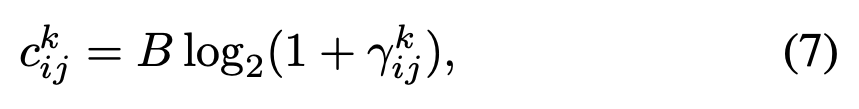
\includegraphics[scale=0.4]{figures/eq7.png}
                    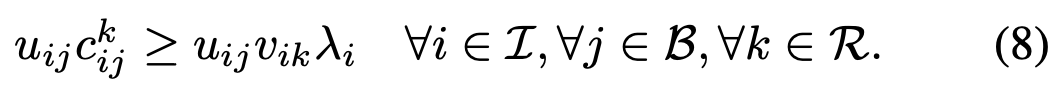
\includegraphics[scale=0.4]{figures/eq8.png}
                \end{center}
        \end{column}
        \end{columns}
    \end{frame}

    \begin{frame}{制約条件9-18}
        \begin{columns}
            \begin{column}[T]{.6\linewidth}
                \begin{itemize}
                    \item 汎化誤差の上界を推定
                    \begin{itemize}
                        \item 汎化誤差は未知のデータに対する予測の誤差
                        \item 上界は実際の集合より大きな数値のこと?
                        % \item 事実上の上限かそれに近いと理解
                    \end{itemize}    
                    \item 汎化誤差を最小化したい
                    \begin{itemize}
                        \item 予測の精度を向上させるのが目的
                        \item 汎化誤差を最小化する式は18
                        \item パラメータはU,VIDに対してBSは0個でもいい
                    \end{itemize}    
                \end{itemize}          
            \end{column}
            \begin{column}[T]{.5\linewidth}
                \begin{center}
                    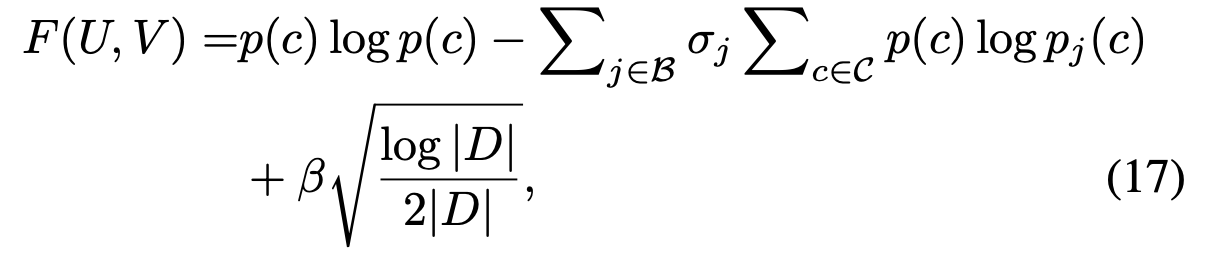
\includegraphics[scale=0.3]{figures/eq17.png}
                    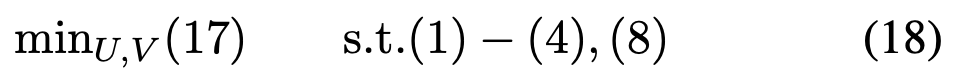
\includegraphics[scale=0.4]{figures/eq18.png}
                \end{center}
        \end{column}
        \end{columns}
    \end{frame}




    \begin{frame}{実験1 数値シミュレーション}
        \begin{columns}
            \begin{column}[T]{.7\linewidth}
                \begin{itemize}
                \item 問題設定
                \begin{itemize}
                    \item ID 20,BS 3,RB 5
                    \item ID, BSは1kmの正方形空間にランダム配置
                    \item IDで生成されるデータの量: $\lambda_{i} = 100|1000$  Kbps
                    \item 学習時間の$T$における総量 50000 データ
                    \item ラベル数は10
                    \item 各IDのラベル分布$p_i (C)$はランダム
                \end{itemize}
                \item 生成データ量を変えて実験
                \item 式17の$\beta$依存性も見た
                \item データの量と分布を確認
                \item 最適化は4,8の制約に従う
                \end{itemize}          
            \end{column}
            \begin{column}[T]{.5\linewidth}
                \begin{center}
                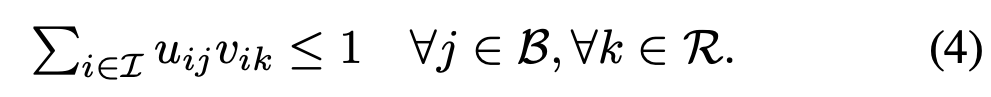
\includegraphics[scale=0.4]{figures/eq4.png}
                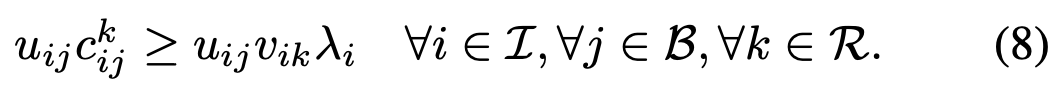
\includegraphics[scale=0.4]{figures/eq8.png}
                \end{center}
            \end{column}
        \end{columns}
    \end{frame}


    \begin{frame}{実験1 数値シミュレーション}
        \begin{columns}
            \begin{column}[T]{.7\linewidth}
                \begin{itemize}
                \item ナイーブ法
                    \begin{itemize}
                        \item IDはランダムに配置
                        \item 最も近いBSに接続
                    \end{itemize}
                \end{itemize}          
            \end{column}
            \begin{column}[T]{.5\linewidth}
            \end{column}
        \end{columns}
    \end{frame}


    \begin{frame}{実験1の結果}
        \begin{columns}
            \begin{column}[T]{.5\linewidth}
                \begin{itemize}
                \item fig2の見方
                    \begin{itemize}
                        \item 星がBS
                        \item 点がID
                        \item 同じ色のBSに接続
                        \item 黒は未接続
                    \end{itemize}
                \end{itemize}    
            \end{column}
            \begin{column}[T]{.5\linewidth}
                \begin{center}
                    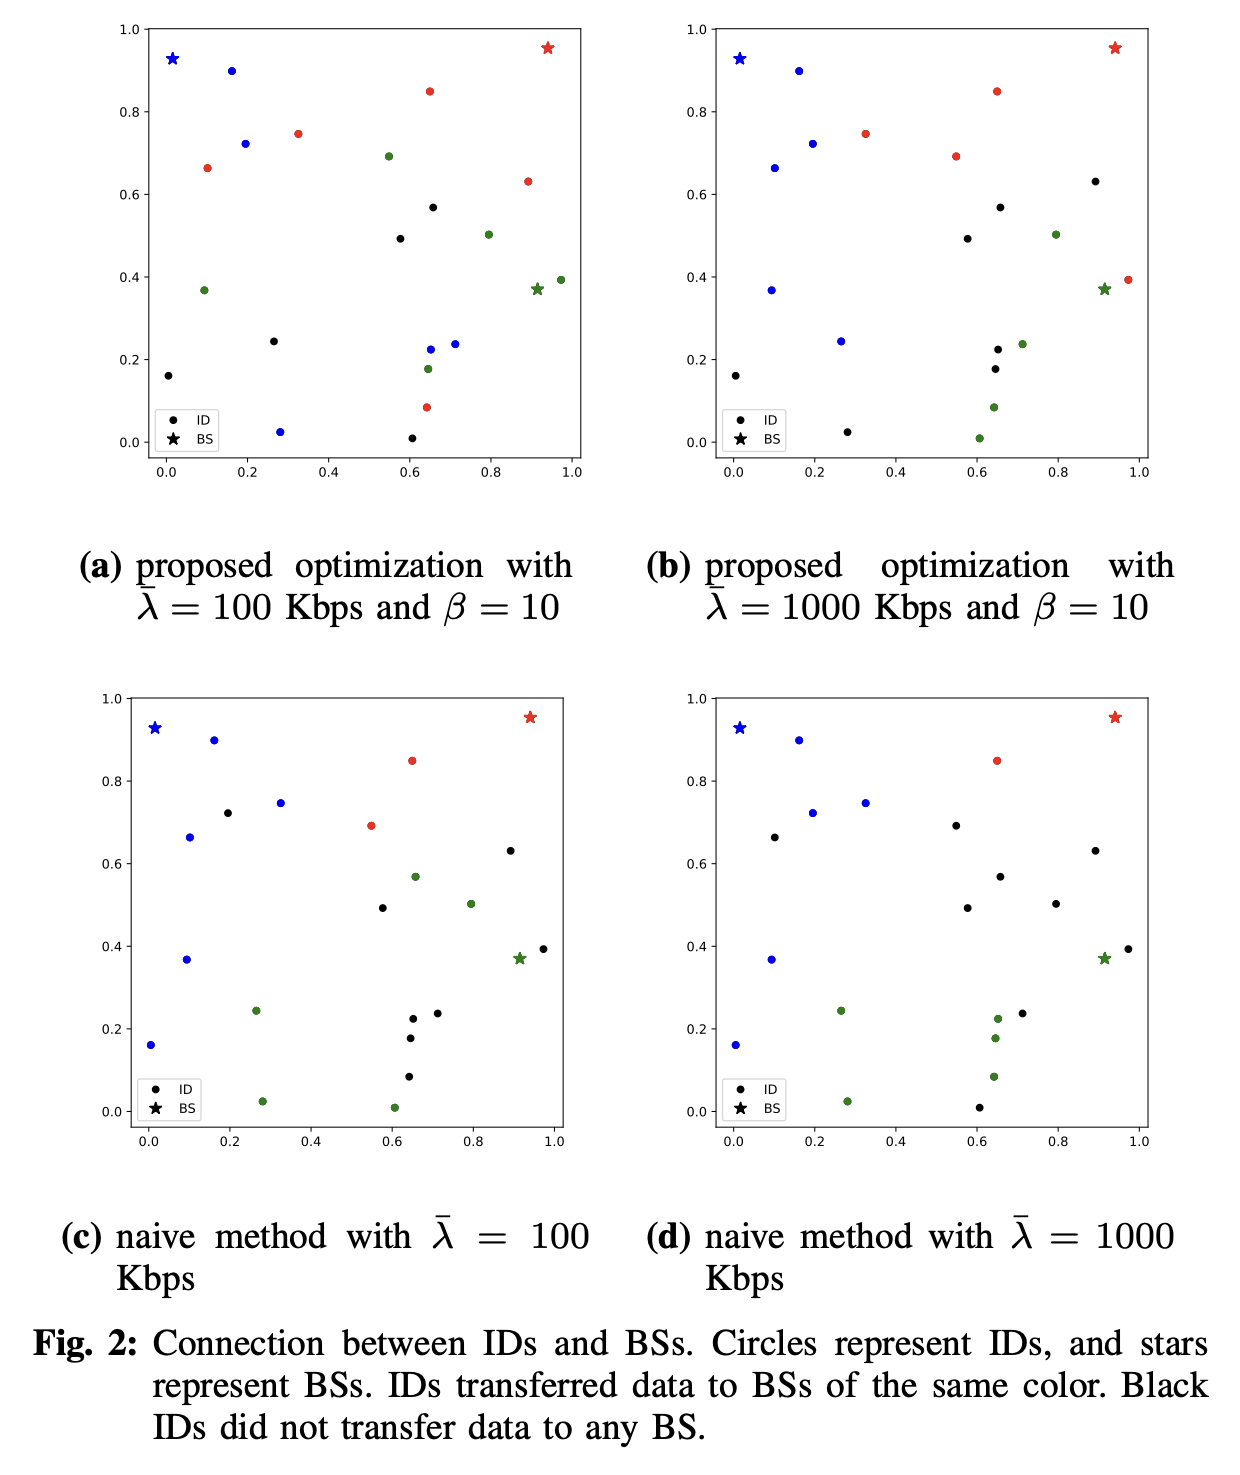
\includegraphics[scale=0.3]{figures/fig-2.png}                    
                \end{center}
                \end{column}
        \end{columns}
    \end{frame}

    \begin{frame}{実験1の結果}
        \begin{columns}
            \begin{column}[T]{.6\linewidth}
                \begin{itemize}
                \item 図a,bの比較
                    \begin{itemize}
                        \item データ生成量の多寡
                        \item aは生成量小
                            \begin{itemize}
                                \item 制約8での送信先の縛りが緩い
                            \end{itemize}   
                        \item bは生成量大
                            \begin{itemize}
                                \item 扱うデータ量が増大
                                \item 制約がより厳しくなる
                                \item 近いBSに送信することが多い
                            \end{itemize}
                        \end{itemize}
                \item 提案手法とナイーブの比較
                    \begin{itemize}
                        \item 提案手法はBSに接続したIDの総量が多い
                        \item 利用したデータの数が多い
                        \item KL(p(c)¦pj (c))が小さい?
                    \end{itemize}
                \end{itemize}    
            \end{column}
            \begin{column}[T]{.5\linewidth}
                \begin{center}
                    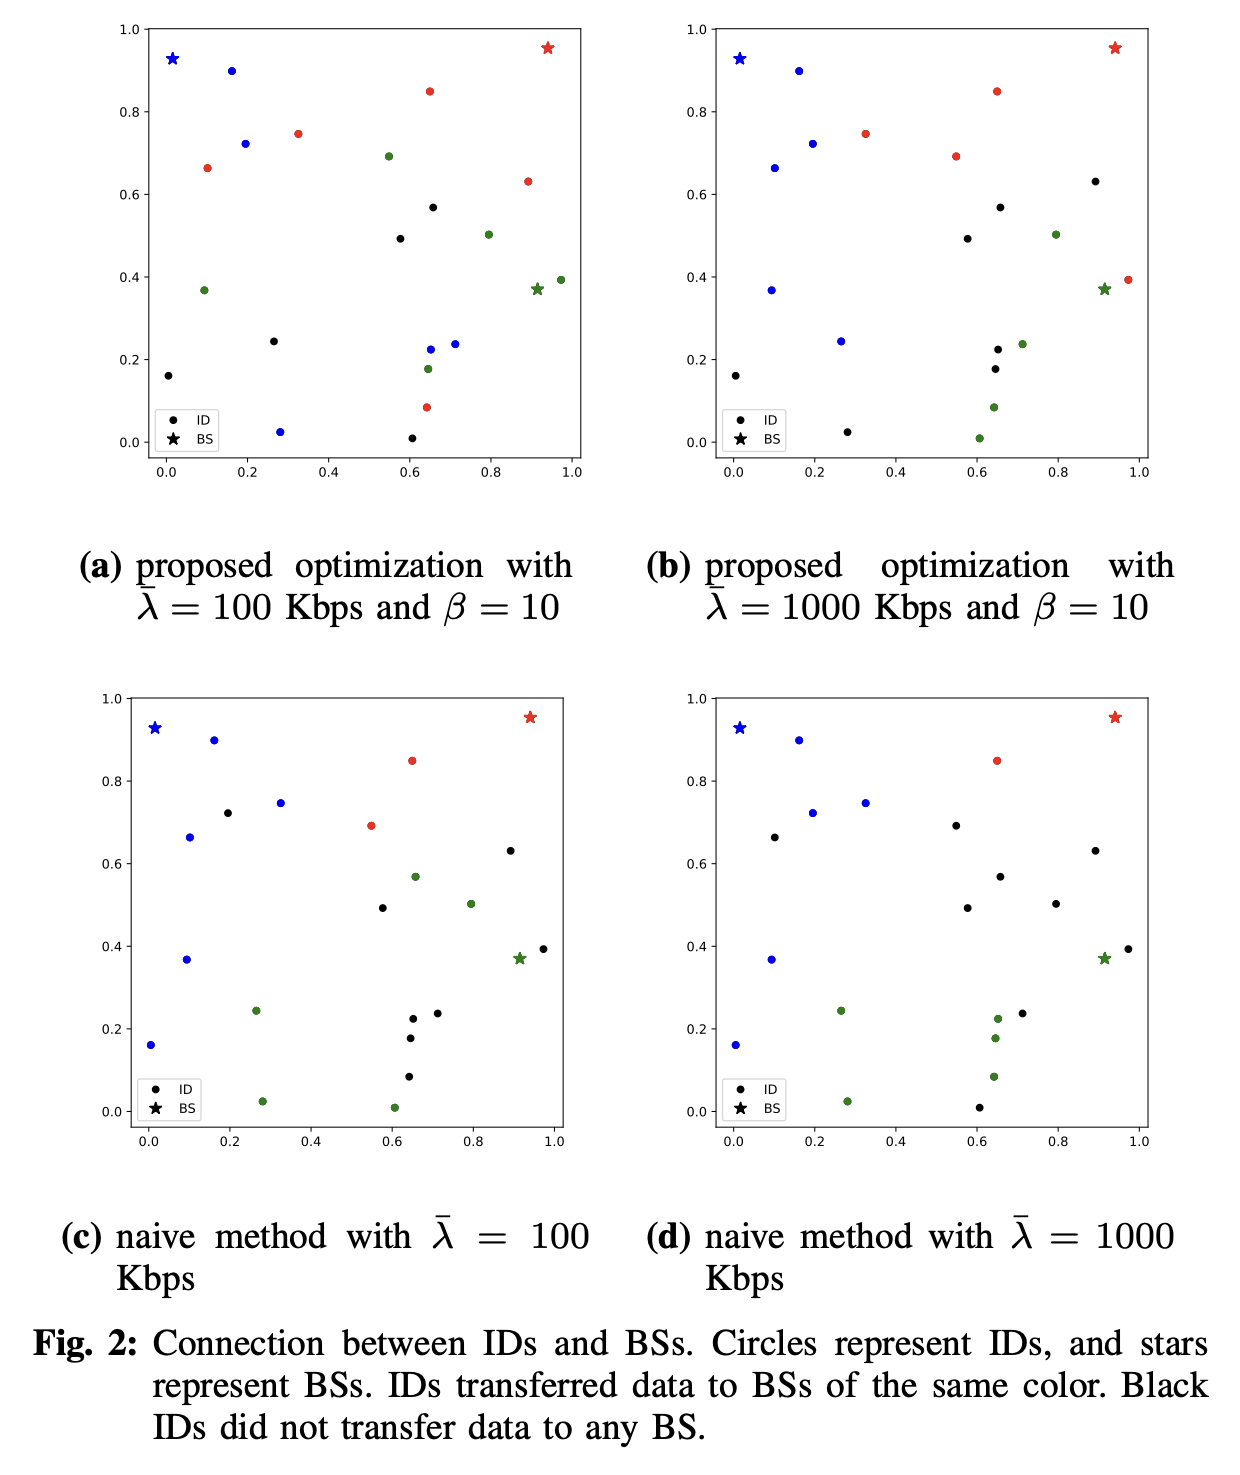
\includegraphics[scale=0.3]{figures/fig-2.png}                    
                \end{center}
                \end{column}
        \end{columns}
    \end{frame}



    \begin{frame}{実験2 深層学習モデル 問題設定}
        \begin{columns}
            \begin{column}[T]{.6\linewidth}
                \begin{itemize}
                    \item データセット
                    \begin{itemize}
                        \item cifar10
                        \item 画像の10クラス分類
                        \item 全部で5万のデータ
                    \end{itemize}
                    \item IDのデータ分布
                    \begin{itemize}
                        \item シミュレーションで決まったλiとpi (c)に従う
                        \item ランダムに選択?
                    \end{itemize}
                    \item 利用したモデル
                    \begin{itemize}
                        \item VGG19
                        \item DenseNet121
                        \item ResNet152
                    \end{itemize}
                \end{itemize}    
            \end{column}
            \begin{column}[T]{.5\linewidth}
                \begin{center}
                    % 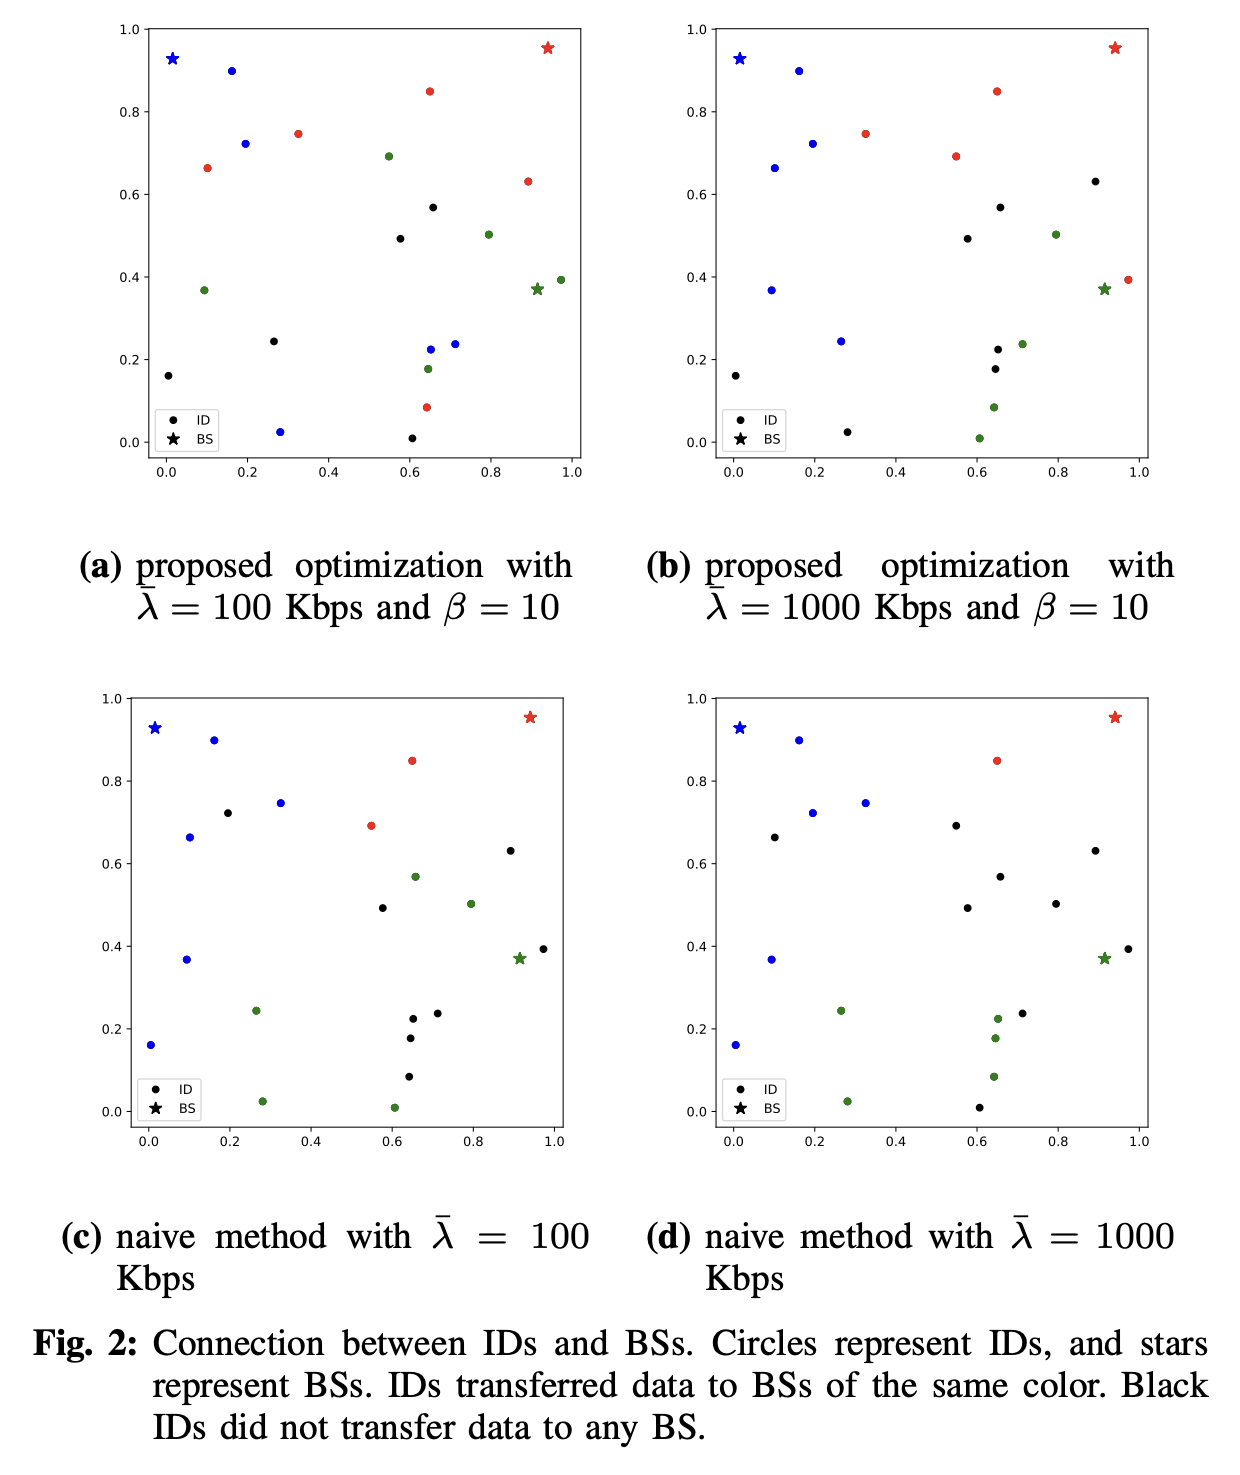
\includegraphics[scale=0.3]{figures/fig-2.png}                    
                \end{center}
                \end{column}
        \end{columns}
    \end{frame}


    \begin{frame}{実験2 深層学習モデル 問題設定}
        \begin{columns}
            \begin{column}[T]{.6\linewidth}
                \begin{itemize}
                    \item FLをFlowerで実装
                    \item FedAVGで集約
                    \item FLの設定
                    \begin{itemize}
                        \item 5つのローカルトレーニング
                        \item 多分五回
                        \item 50エポック
                        \item 一回で50回?
                        \item 50回になるよう繰り返した?
                    \end{itemize}
                \end{itemize}    
            \end{column}
            \begin{column}[T]{.5\linewidth}
                \begin{center}
                    % 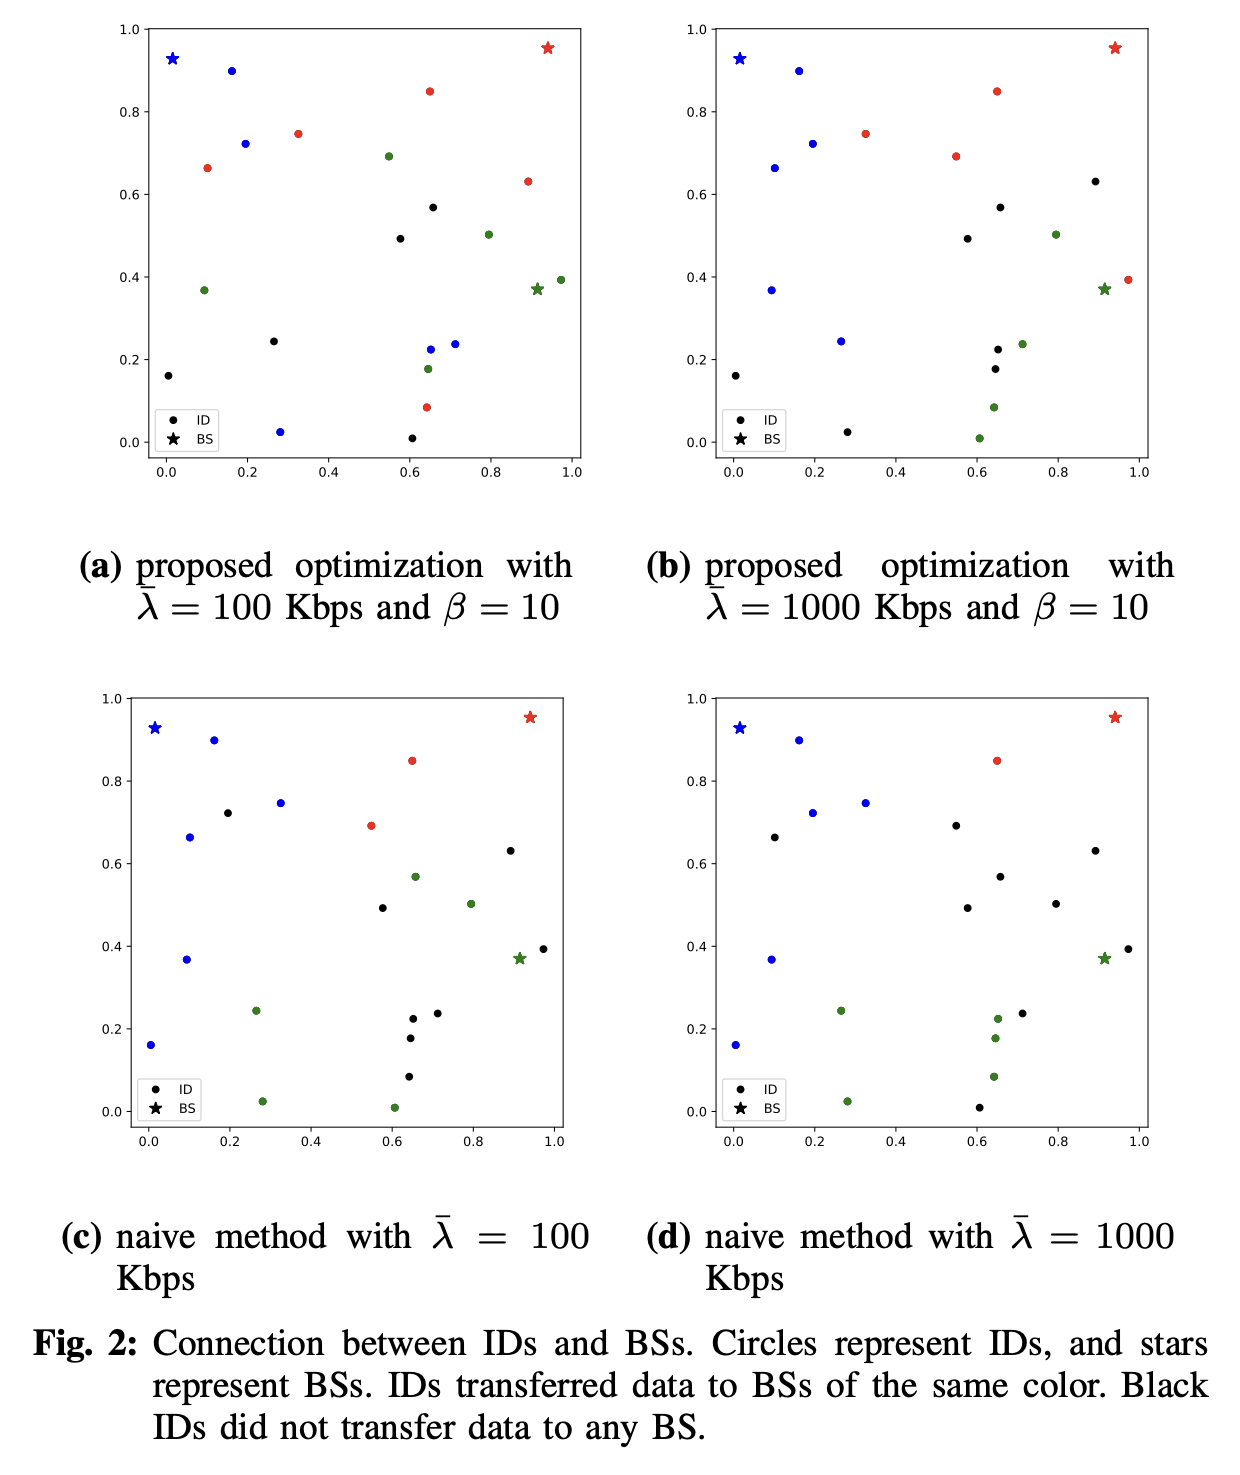
\includegraphics[scale=0.3]{figures/fig-2.png}                    
                \end{center}
                \end{column}
        \end{columns}
    \end{frame}

    \begin{frame}{実験2 結果}
        \begin{columns}
            \begin{column}[T]{.5\linewidth}
                \begin{itemize}
                    \item データセット
                    \item 精度の差が出た理由
                        \begin{itemize}
                            \item 100の時
                                \begin{itemize}
                                    \item 2ポイントほど差があった
                                    \item 制約が緩いため
                                    \item 最良のデータ転送が行えた
                                    \item 量と分布が最適になる転送?
                                \end{itemize}    
                                \item データ生成量1000の時
                                \begin{itemize}
                                    \item 精度はほぼ同じ
                                    \item データが増え,制約が厳しく
                                \end{itemize}    
                        \end{itemize}
                    % \item 最適化の意図はなんだったっけ?
                    % \item 制約下でも輻輳を起こさずにFLを行える?
                    \item $\beta$もKLも最適化で重要
                    \item モデルの構造に依存する?
                \end{itemize}    
            \end{column}
            \begin{column}[T]{.5\linewidth}
                \begin{center}
                    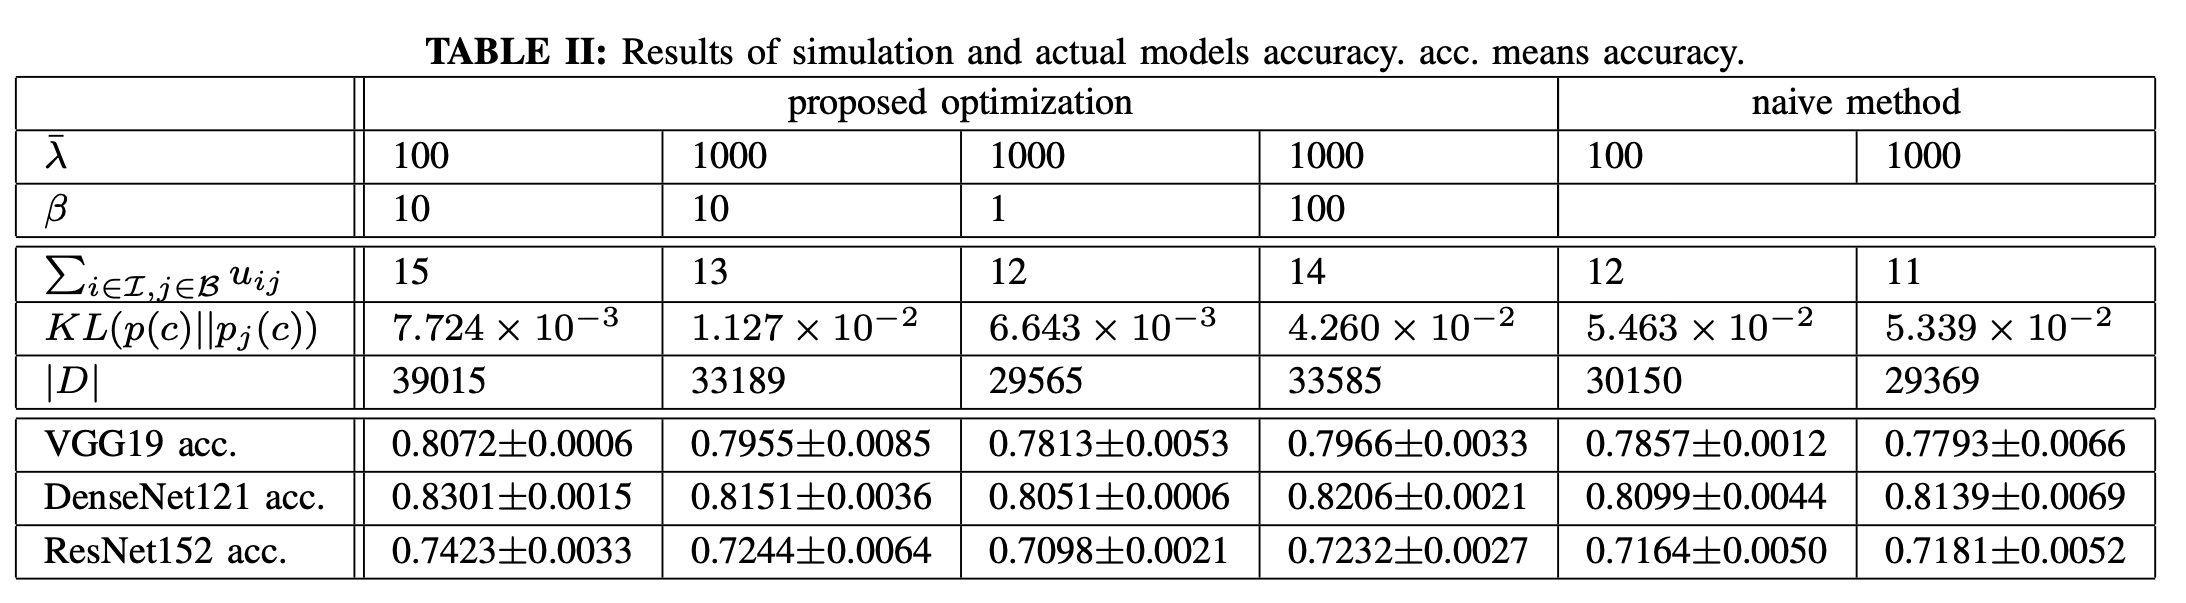
\includegraphics[scale=0.3]{figures/table.png}                    
                \end{center}
                \end{column}
        \end{columns}
    \end{frame}


    \begin{frame}{実験2 結果}
        \begin{center}
            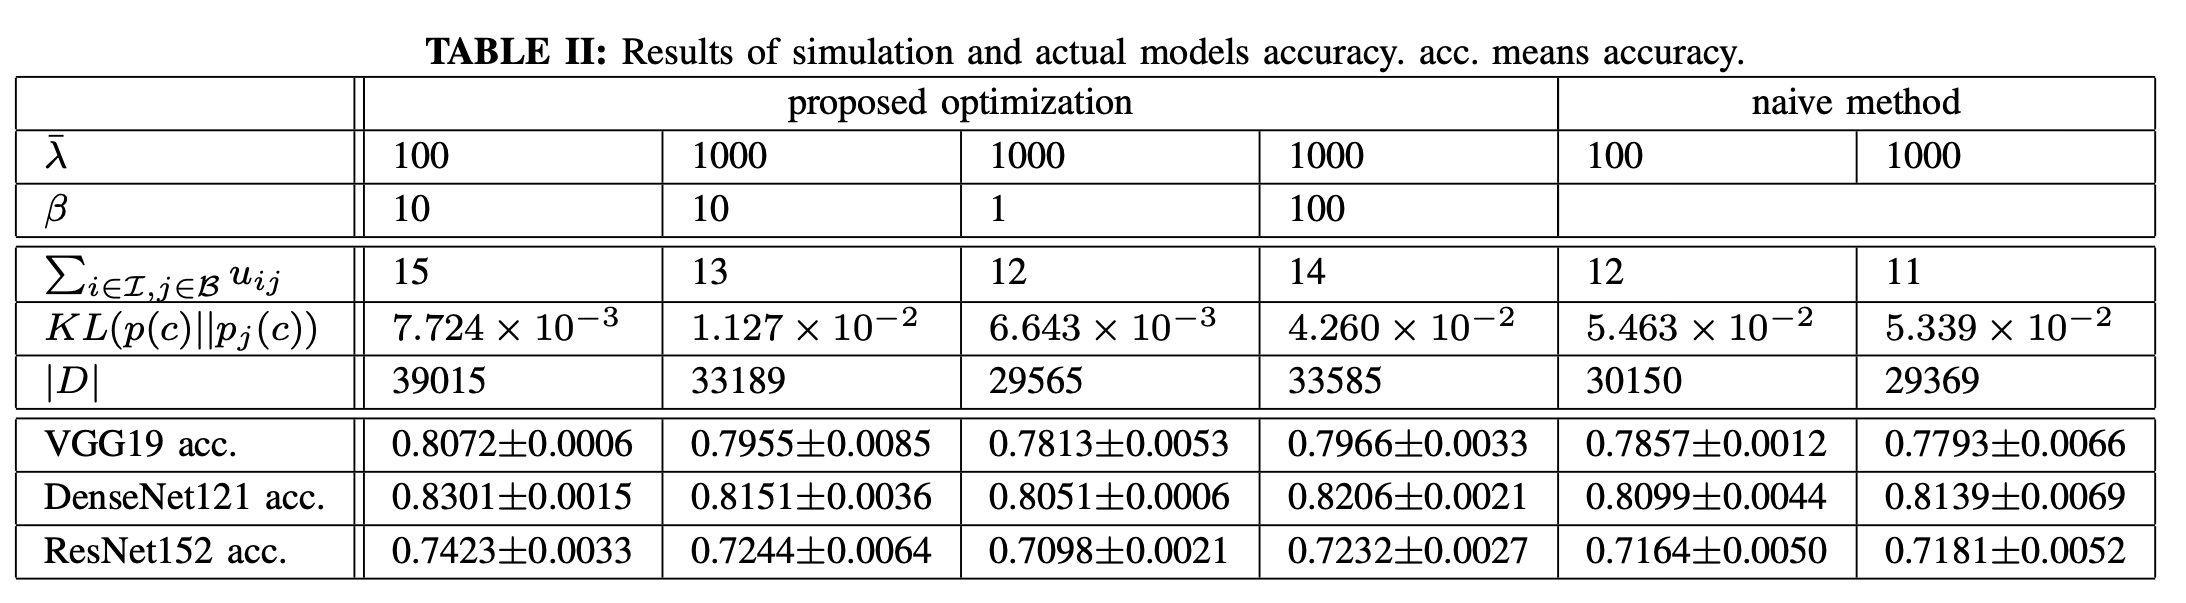
\includegraphics[scale=0.4]{figures/table.png}                    
        \end{center}
    \end{frame}





    \section{4. 知見}
    \begin{frame}{得られた結果,知見}
        \begin{columns}
            \begin{column}{.8\linewidth}
                \begin{itemize}
                   \item 提案手法はナイーブと比べて精度を改善
                   \begin{itemize}
                    \item いずれの実験でも改善された
                    \begin{itemize}
                        \item 実験2は平均値で観察
                        \item 詳細な設定はまだ見ていない
                    \end{itemize}
                    \item データ転送の最適化でFLの精度が向上
                    \item IDからBSにデータを送信しFLを行うシナリオにおいて
                    \begin{itemize}
                        \item 提案手法は制約条件の下,データ量と分布が最適になるようデータを送信
                        \item データ転送の観点から精度の向上が実現
                    \end{itemize}
                \end{itemize}
                \end{itemize}          
            \end{column}
        \end{columns}
    \end{frame}


    \section{5. 他}
    \begin{frame}{分かっていない/気になる点}
        \begin{columns}
            \begin{column}{.8\linewidth}
                \begin{itemize}
                    \item 用語など
                    \begin{itemize}
                        \item 遺伝的アルゴリズム
                        \item 最適化の式
                    \end{itemize}
                    \item 精度がナイーブより高いことの意味
                    \begin{itemize}
                        \item 制約を守った上で精度が高いのが偉い?
                        \item 帯域幅の制約を守るFLが先??
                        \item 守った上で精度が出せたのが偉いのか,精度が出せるのは当たり前なのか
                    \end{itemize}
                    \item 数値シミュレーション
                    \begin{itemize}
                        \item 最適化手法は式17を小さくするために多数接続
                        \item BSに接続するIDの数が増えると良いらしい
                        \item $\beta$依存性の議論
                    \end{itemize}
                \end{itemize}          
            \end{column}
        \end{columns}
    \end{frame}

    \begin{frame}{分かっていない/気になる点}
        \begin{columns}
            \begin{column}{.8\linewidth}
                \begin{itemize}
                    \item より複雑なモデルでの検証
                    \item ID,BS間の具体的な通信
                    \item FLについて,バッテリー制約も同時に満たせないか
                    \item モデル転送も考慮できないか
                \end{itemize}          
            \end{column}
        \end{columns}
    \end{frame}



\end{document}